\section{Исследовательская часть}

В данном разделе будет проведено исследование разработанной программы. Будет верифицированна её работоспособность в различных конфигурациях системы. Также будут выявлены ограничения применимости приложения. Результаты всех экспериментов будут сопровождены выводами.  

\subsection{Постановка задачи}
С целью проверки работоспособности разработанного метода требуется сравнить стоимости начального и оптимизированного плана при различных размерностях транспортной системы.

Также необходимо произвести замеры среднего времени работы программы при разном количестве пунктов маршрутов для определения ограничений его применимости.

С целью определения закономерностей работы метода будут проведены исследования зависимости общей стоимости маршрутов от следующих параметров:

\begin{enumerate}
	\item вместительность грузовика;
	\item средняя удалённость пунктов маршрута от стоянки;
\end{enumerate}

\subsection{Генерация транспортной системы}
Для проведения экспериментов необходимо иметь описания большого количества (не менее ста) транспортных систем. Собрать большое количество реальных данных крайне затруднительно. Поэтому более предпочтительной является генерация случайной транспортной системы.

При генерации сети в первую очередь с помощью библиотеки networkx создаётся случайный граф. Полученные позиции вершин и их наличие рёбер между ними используется для создания дорог в транспортной системе. После этого узлам графа случайным образом сопоставляется роль пункта, набор продуктов в заказе или запасах. Пример использования сгенерированной системы приведён на рисунке \ref{demo:routes2}.

\subsection{Проведение экспериментов}

\subsubsection{Характеристики вычислительной техники}
Эксперименты проводились на персональном компьютере со следующими характеристиками.

\begin{itemize}
	\item Операционная система --- Windows 10, 64-разрядная.
	\item Процессор --- AMD Ryzen 5 5500U with Radeon Graphics 2.10 GHz.
	\item Оперативная память --- 8,00 ГБ.
\end{itemize}

\subsubsection{Исследование работы алгоритма}
Метод потенциалов является многоитерационным, поэтому имеется возможность пронаблюдать изменение системы на каждом шаге и проанализировать за счёт чего достигается более оптимальный план. 

В данном \, эксперименте будет исследованна \, зависимость стоимости \, маршрутов, их количества, средней длине и средней загруженности от текущей итерации оптимизации. Результат проведённого эксперимента изображён в виде графиков на рисунке \ref{exp:iter100}. В исследовании использовались случайные транспортные системы с размерностями в 100 и 200 пунктов маршрута.

\begin{figure}[h!]
	\begin{center}
		{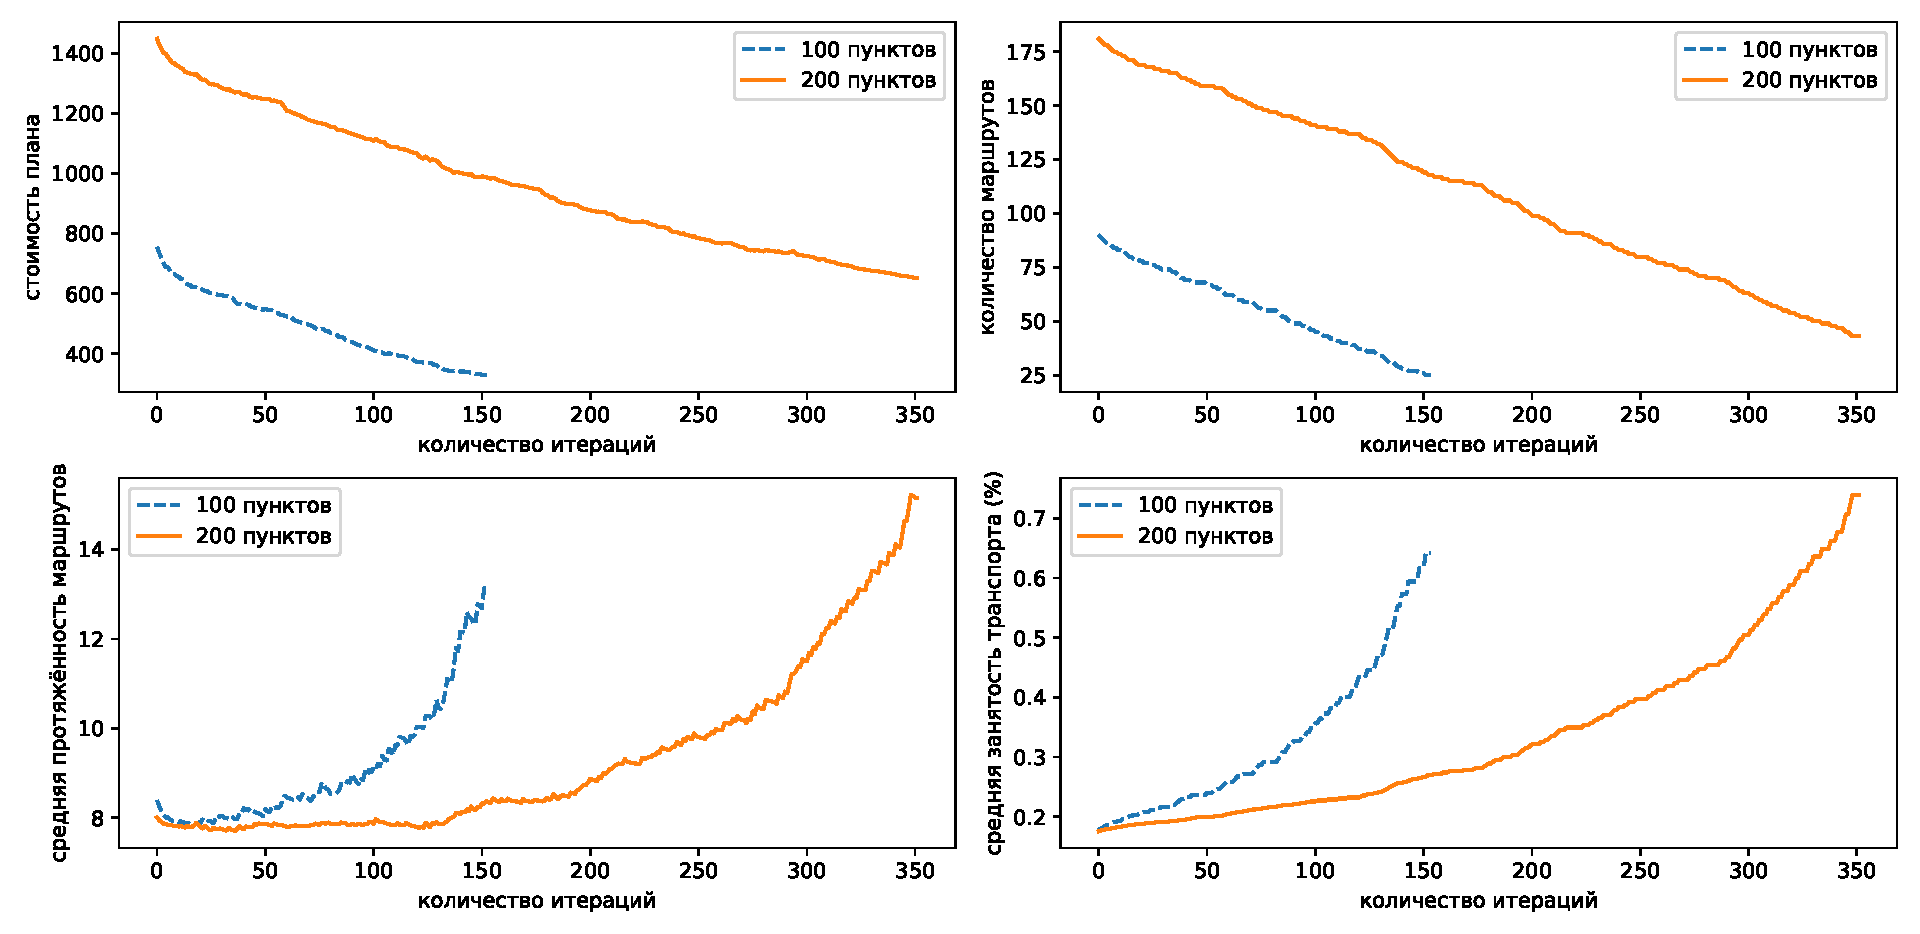
\includegraphics[scale=0.53, angle=0, page=1]{research/detailed_report.pdf}}
		\caption{Исследование работы алгоритма}
		\label{exp:iter100}
	\end{center}
\end{figure}

Из данного графика можно сделать вывод о том, что главным образом снижение стоимости достигается за счёт снижения общего числа маршрутов посредством продления и распределения груза на другие маршруты. Также можно отметить, что данные закономерности не зависят от размера транспортной сети.

\subsubsection{Сравнение плана до и после оптимизации}
Главным показателем корректности реализованного метода является наличие оптимизации. Оно выражается в том, что конечный план должен обладать меньшей суммарной стоимостью для всех маршрутов по сравнению с начальным, опорным планом. 

Чтобы установить выполнение данного условия в общем случае, в данном эксперименте были использованы случайно созданные транспортные сети размером от 20 до 180 пунктов. Измерения для каждой размерности проводятся многократно для усреднения полученных значений. Результат проведённого эксперимента изображён на графике, на рисунках \ref{exp:cmp} -- \ref{exp:cmp2}.

\begin{figure}[h!]
	\begin{center}
		{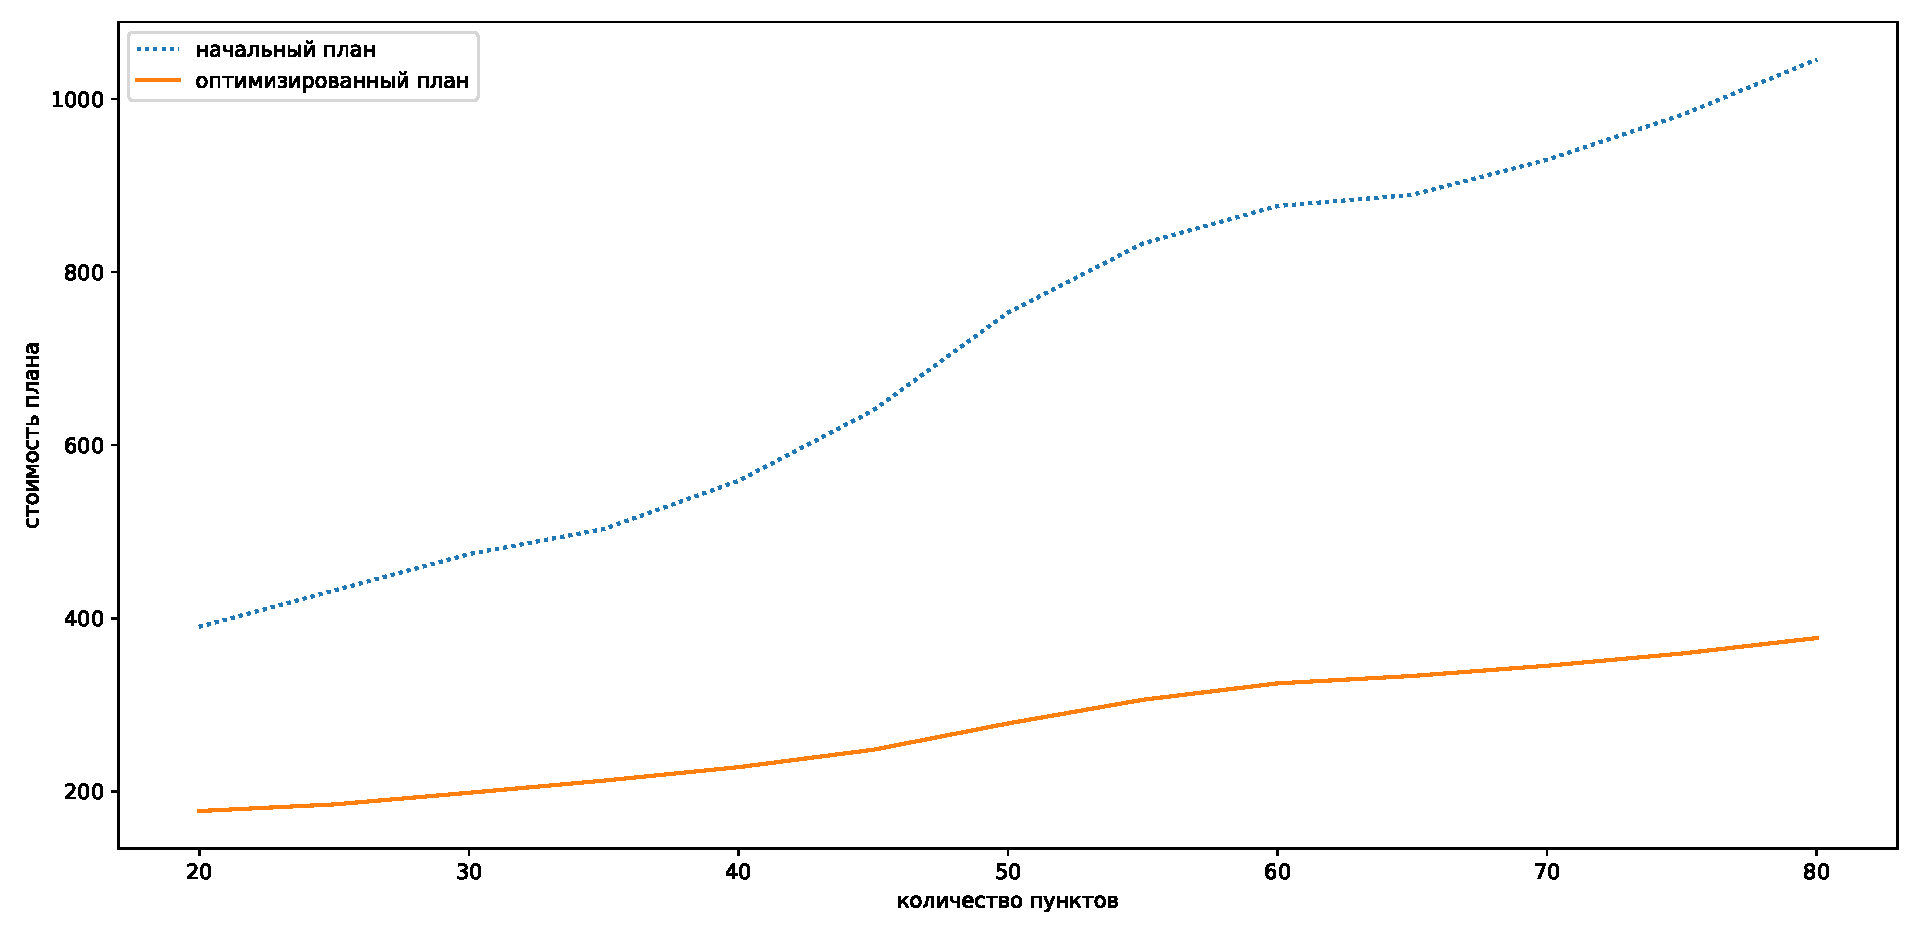
\includegraphics[scale=0.5, angle=0, page=1]{research/cmp.pdf}}
		\caption{Сравнение стоимостей плана до и после оптимизации}
		\label{exp:cmp}
	\end{center}
\end{figure}

\begin{figure}[h!]
	\begin{center}
		{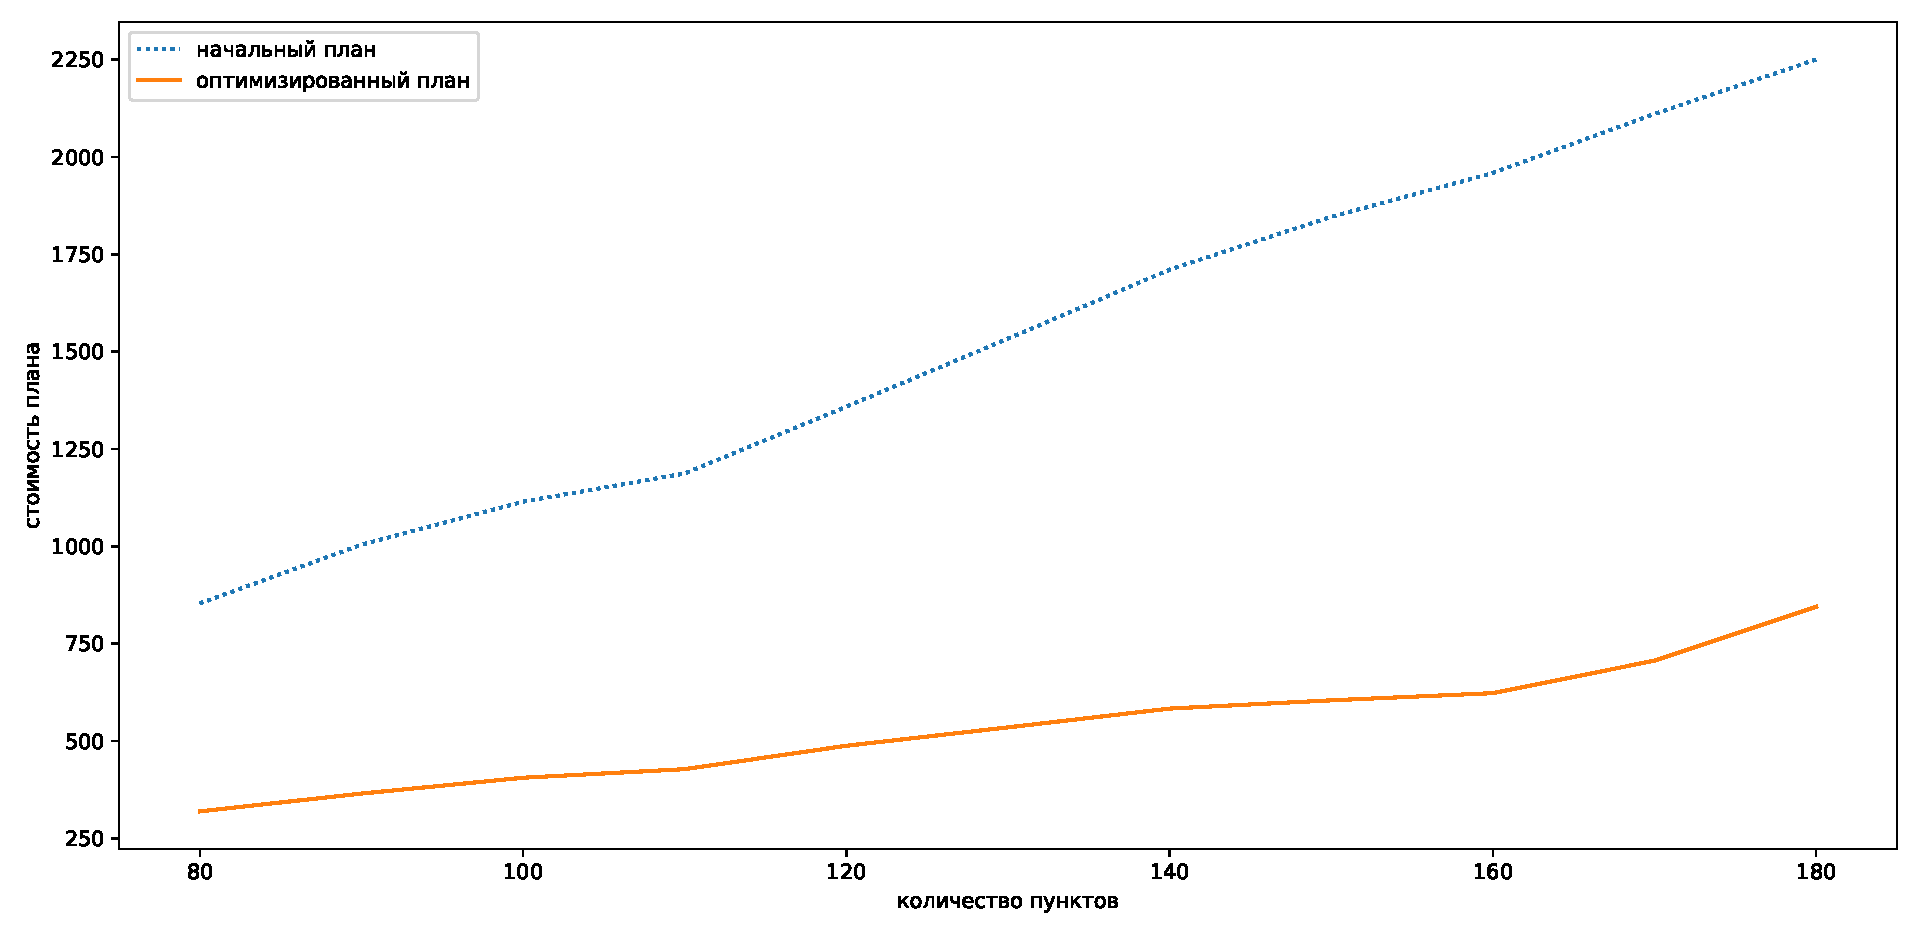
\includegraphics[scale=0.5, angle=0, page=1]{research/cmp2.pdf}}
		\caption{Сравнение стоимостей плана до и после оптимизации (продолжение)}
		\label{exp:cmp2}
	\end{center}
\end{figure}

\pagebreak
Результаты эксперимента показывают, что при любом рассмотренном размере оптимизация опорного плана сокращает стоимость грузоперевозок как минимум вдвое, из чего можно заключить, что метод работоспособен.

\subsubsection{Определение ограничений программы}
Основным ограничением в работе программы может являться рост времени её исполнения при увеличении размерности системы. Для определения существенности данного ограничения следует провести эксперимент по установлению зависимости времени обработки входных данных от их размера.

Для этого будут использованы случайно сгенерированные транспортные системы размером от 20 до 250 узлов. Результат проведённого эксперимента сведён в график, изображённый на рисунке \ref{exp:timing}.

\begin{figure}[h!]
	\begin{center}
		{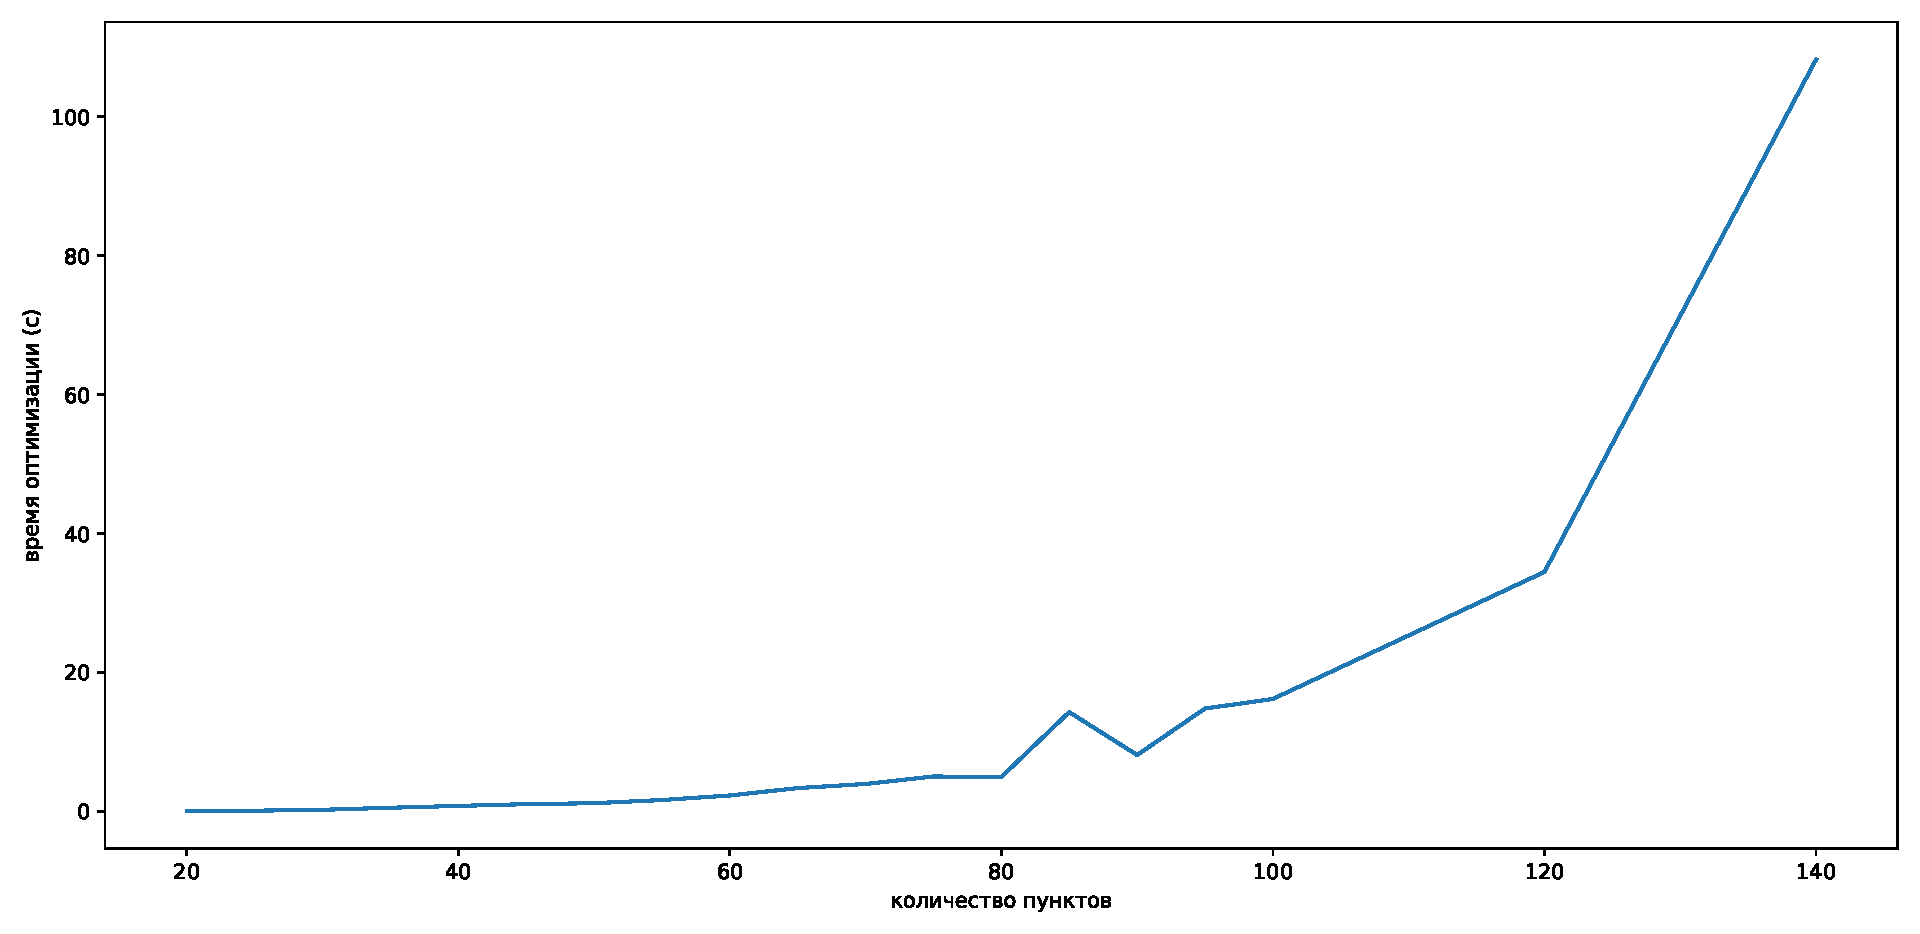
\includegraphics[scale=0.5, angle=0, page=1]{research/timing.pdf}}
		\caption{Зависимость времени работы от размерности}
		\label{exp:timing}
	\end{center}
\end{figure}

Из графика можно сделать вывод о том, что характер роста функции является нелинейным. При размере сети менее 50 пунктов время оптимизации составляет менее одной секунды. Большее количество узлов приводит к значительному росту времени обработки. Можно сделать вывод о том, что программа завершает оптимизацию за приемлемое время (не более 100 секунд) в диапазоне исследованных размерностей. 

Ввиду того, что сети подобного масштаба едва ли могут встретиться на практике, а также учитывая допустимость сравнительно длительного времени работы программы, полученные характеристики можно считать приемлемыми для выполнения поставленной задачи.

\subsubsection{Выявление закономерностей работы системы}
Разработанная программа позволяет моделировать поведение транспортной системы при изменении некоторых параметров. Рассмотрим некоторые из них.

В данном эксперименте изучается влияние вместительности грузовика на стоимость грузоперевозок. Размер системы принят равным 50 пунктам. Средний заказ имеет объём в 1м$^3$. Результат эксперимента приведён на рисунке \ref{exp:truck_vol}.

\begin{figure}[h!]
	\begin{center}
		{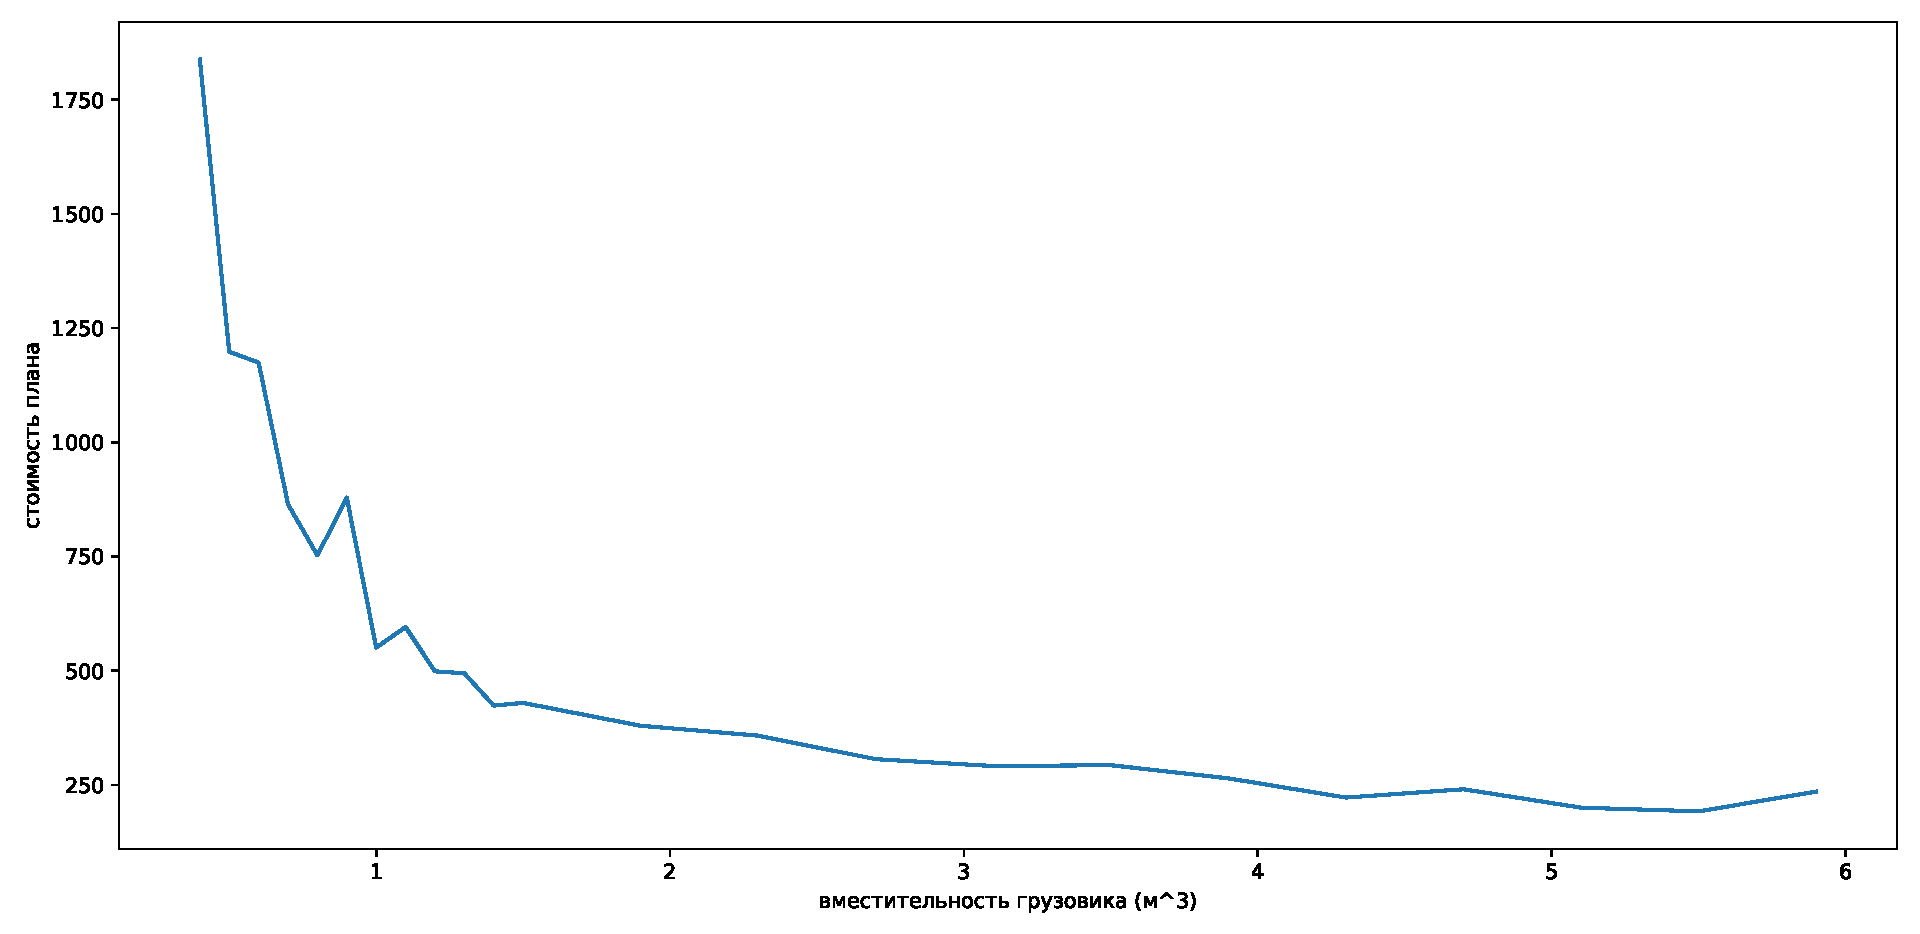
\includegraphics[scale=0.5, angle=0, page=1]{research/truck_vol.pdf}}
		\caption{Зависимость стоимости маршрутов от вместительности грузовиков}
		\label{exp:truck_vol}
	\end{center}
\end{figure}

Из данного графика видно, что использование грузовиков меньше объёма одного заказа невыгодно. 

\pagebreak
Так как все маршруты начинаются и завершаются на стоянке, её положение относительно других пунктов может существенно влиять на маршруты. На рисунке \ref{exp:parking_dist} изображен эксперимент по выявлению зависимости стоимости маршрутов от среднего расстояния до стоянки. 

\begin{figure}[h!]
	\begin{center}
		{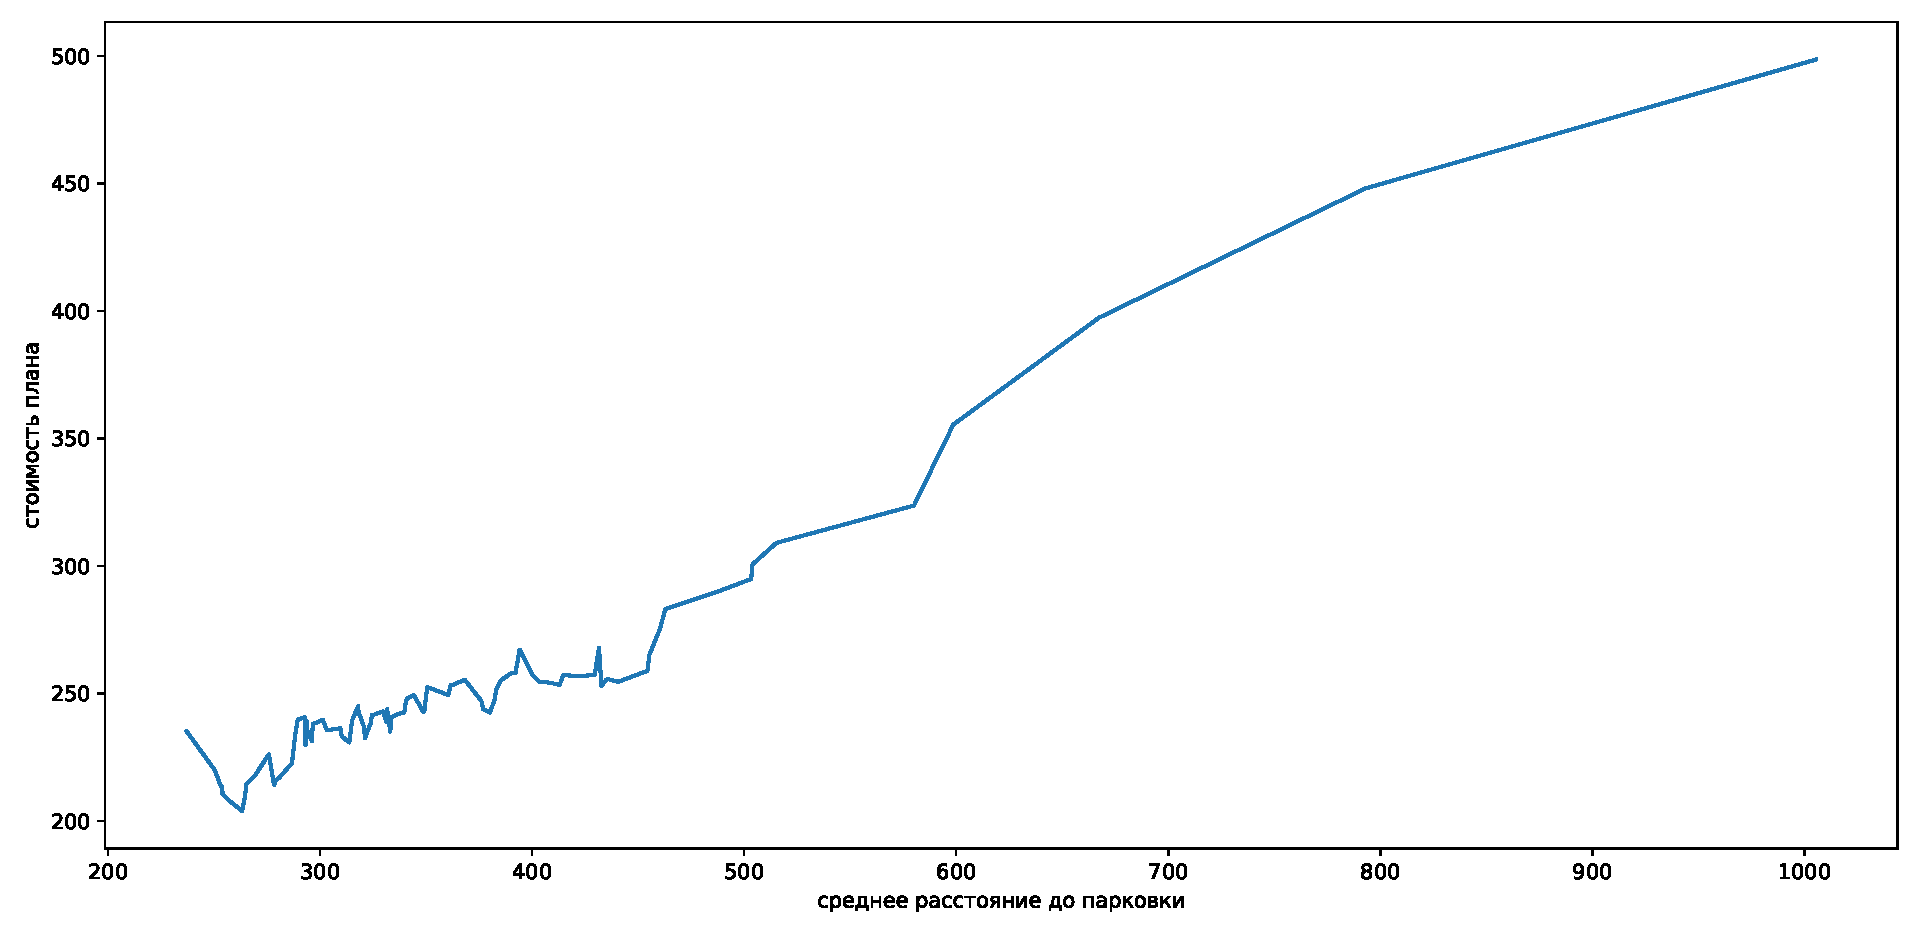
\includegraphics[scale=0.5, angle=0, page=1]{research/parking_dist.pdf}}
		\caption{Зависимость стоимости маршрутов от удалённости стоянки}
		\label{exp:parking_dist}
	\end{center}
\end{figure}

Получившийся график не является монотонным, так как средняя удалённость считается по случайно сгенерированной системе, в которой могут иметься иные параметры, влияющие на результат. Однако, с ростом среднего расстояния видна тенденция на рост общей стоимости. 

Из этих экспериментов можно сделать вывод о том, что в целях оптимизации издержек, транспортной компании следует минимизировать расстояние от стоянки до потребителей и использовать транспорт, способный вместить в себя по крайней мере несколько целых заказов.

\subsection*{Вывод}
В данном разделе были описаны цели и планы проводимых экспериментов. В их рамках были проанализированны изменения различных параметров системы при работе алгоритма оптимизации, экспериментально обоснована работоспособность метода. Были выявленны ограничения для использования разработанной программы, а также некоторые закономерности работы транспортной системы, на основе которых были предложены рекомендации по организации грузоперевозок. 

\pagebreak